\def\year{2018}\relax
%File: formatting-instruction.tex
\documentclass[letterpaper]{article} %DO NOT CHANGE THIS
\usepackage{aaai18}  %Required
\usepackage{times}  %Required
\usepackage{helvet}  %Required
\usepackage{courier}  %Required
\usepackage{url}  %Required
\usepackage{graphicx}  %Required
\usepackage{amsmath,amsfonts}
\usepackage{tabu}
\usepackage{subfigure}
\newcommand\norm[1]{\left\lVert#1\right\rVert}
\def \y {\mathbf{y}}
\def \x {\mathbf{x}}
\def \Y {\mathbf{Y}}
\def \X {\mathbf{X}}
\def \w {\mathbf{w}}
\def \v {\mathbf{v}}
\def \V {\mathbf{V}}
\def \Z {\mathbf{Z}}
\def \A {\mathbf{A}}
\def \z {\mathbf{z}}
\def \P {\mathbf{P}}
\frenchspacing  %Required
\setlength{\pdfpagewidth}{8.5in}  %Required
\setlength{\pdfpageheight}{11in}  %Required
%PDF Info Is Required:
  \pdfinfo{ 
/Title (Robust and Effective Factorization Machines)
/Author (Anonymous)}
\setcounter{secnumdepth}{0}  
 \begin{document}
% The file aaai.sty is the style file for AAAI Press 
% proceedings, working notes, and technical reports.
%
\title{Robust and Effective Factorization Machines}
\author{Anonymous
}
\maketitle

\section{Optimization Algorithm}
The original objective for classsification task takes the form:
\begin{small}
\begin{align}
	\min_{\w \in \mathbf{R}^d,\Z \in \mathbf{S}_{+}^{d \times d}} &\sum_{i=1}^{n}e_i(\max\{\max(y_i(\w^\top\x_i+\langle\Z, \x_i\x_i^\top\rangle),0)-\epsilon_1,0\})^2 \nonumber \\ 
	&+ \frac{\alpha}{2}\norm{\w}^2 + \sum_s\min\{\lambda_s^2, \epsilon_3\},
\end{align}
\end{small}
\begin{align}
e_i=
	\begin{cases}
	\frac{1}{2error},& 0 < error \leq \epsilon_2;\\
	0, & otherwise
	\end{cases}\nonumber
\end{align}
where $error=\max(y_i(\w^\top\x_i+\langle\Z, \x_i\x_i^\top\rangle),0)-\epsilon_1$\\
The subgradient with respect to $\Z$ is
\begin{align}
\bigtriangledown_{\Z, I} = \sum_{i=1}^{b}{\x_i\x_i^\top} + \beta\P_M\P_M^\top\Z 
\end{align}
To incrementally calculate the SVD of $\Z - \eta \bigtriangledown_{\Z,I}$. Let the symmetric and low rank matrix $\Z$ has rank $k$ and its economy SVD is $\Z=\P_k\Sigma_k\P_k^\top$.
As matrix $\bigtriangledown_{\Z,I}$ is symmetric and low rank, we can represent it as $\A \A^\top$.
\begin{align}
\bigtriangledown_{\Z,I}&=\X\X^\top + \beta\P_M\P_M^\top\Z \\ \nonumber
\end{align}

\section{Experiments}
In this section, we empirically investigate whether our proposed RobFM method can achieve better and robust performance compared to original factorization machine model with fixed rank on benchmark datasets.
\subsection{Experimental Testbeds and Setup}
We conduct our experiments on four public datasets. Table \ref{tab0} gives a brief summary of these datasets. All the datasets are normalized to have zero mean and unit variance in each dimension. To make fair comparison, all the algorithms are conducted over $5$ experimental runs of different random permutations. We apply hinge loss for training and evaluate the performance of our proposed methods for classification task by measuring accuracy and hinge loss. For parameter settings, we perform grid search to choose the best parameters for each algorithm on the training set.
\begin{table}[htb]
	\centering
		\begin{tabular} {|l|c|c|c|c|}
			\hline
			Dataset & \#Training & \#Test & \#Feature   & \#class \\
			\hline
			phishing	& 7370		& 3685		& 68	& 2\\
			w8a			& 49749		& 14951		& 300	& 2\\
			protein		& 17766		& 6621		& 357	& 3\\
			IJCNN       & 49990     & 91701     & 22	& 2\\
			Covtype		& 387342	& 193670	& 54	& 2\\
			MNIST		& 60000		& 10000		& 784	& 10\\
			\hline
		\end{tabular}
	\caption{Summary of datasets used in our experiments.}
	\label{tab0}
\end{table}

\subsection{Experimental Results}
\begin{table*}
	\begin{tabu} to \textwidth {|X[c]| X[c]| X[c]| X[c]|}
		\hline
		phishing           & Train loss & Test loss & Acc(\%)  \\
		\hline
		\textbf{LR} 	 &$\pm$  &$\pm$  &  $\pm$    \\ \hline
		\textbf{SVM} 	 &0.1451$\pm$0.0002  &0.1590$\pm$0.0058  &  93.26 $\pm$ 0.30    \\ \hline
		\textbf{FM} 	  	&0.1397$\pm$0.0002 &0.1534$\pm$0.0006  &93.35 $\pm$ 0.10   \\ \hline
		\textbf{RobFM-IncSVD} 	 &$\pm$  &$\pm$  &  $\pm$    \\ \hline
		\textbf{RobFM}   	&\textbf{0.1145$\pm$0.0004} &\textbf{0.1357$\pm$0.0051}  &\textbf{94.59 $\pm$ 0.33}   \\ \hline
		w8a               & Train loss & Test loss & Acc(\%) \\
		\hline
		\textbf{LR} 	 &$\pm$  &$\pm$  &  $\pm$    \\ \hline
		\textbf{SVM} 	 &0.0305$\pm$0.0006  &0.0316$\pm$0.0003  & 98.65 $\pm$ 0.02   \\ \hline
		\textbf{FM} 	 &0.0234$\pm$0.0010  &0.0245$\pm$0.0002  & 98.86 $\pm$ 0.07   \\ \hline
		\textbf{RobFM-IncSVD} 	 &$\pm$  &$\pm$  &  $\pm$    \\ \hline
		\textbf{RobFM}   &\textbf{0.0178$\pm$0.0007}  &\textbf{0.0190$\pm$0.0003}  &\textbf{99.10 $\pm$ 0.06}  \\ \hline
		\hline
		protein               & Train loss & Test loss & Acc(\%) \\
		\hline
		\textbf{LR} 	 &$\pm$  &$\pm$  &  $\pm$    \\ \hline
		\textbf{SVM} 	 &1.5369$\pm$0.0002  &1.5198$\pm$0.0014  & 68.61 $\pm$ 0.07    \\ \hline
		\textbf{FM} 	 &1.3757$\pm$0.0002  &1.4668$\pm$0.0016  &69.21 $\pm$ 0.10    \\ \hline
		\textbf{RobFM-IncSVD} 	 &$\pm$  &$\pm$  &  $\pm$    \\ \hline
		\textbf{RobFM}   &\textbf{$\pm$}  &\textbf{$\pm$}  &\textbf{$\pm$}  \\ \hline
		\hline
		IJCNN              & Train loss & Test loss & Acc(\%) \\
		\hline
		\textbf{LR} 	 &$\pm$  &$\pm$  &  $\pm$    \\ \hline
		\textbf{SVM} 	 &0.1770$\pm$0.0004  &0.1843$\pm$0.0003  & 91.35 $\pm$ 0.02    \\ \hline
		\textbf{FM} 	 &0.0930$\pm$0.0005  &0.0955$\pm$0.0004  & 96.66 $\pm$ 0.09 \\ \hline
		\textbf{RobFM-IncSVD} 	 &$\pm$  &$\pm$  &  $\pm$    \\ \hline
		\textbf{RobFM} 	 &\textbf{0.0712$\pm$0.0001}  &\textbf{0.0744$\pm$0.0013}  & \textbf{97.83 $\pm$ 0.15}  \\ \hline
		\hline
		Covtype           & Train loss & Test loss & Acc(\%)  \\
		\hline
		\textbf{LR} 	 &$\pm$  &$\pm$  &  $\pm$    \\ \hline
		\textbf{SVM} 	 &0.6080$\pm$0.0003  &0.6102$\pm$0.0002  & 68.76 $\pm$ 0.06    \\ \hline
		\textbf{FM} 	  	&0.5111$\pm$0.0001 &0.5088$\pm$0.0030  &77.31 $\pm$ 0.10   \\ \hline
		\textbf{RobFM-IncSVD} 	 &$\pm$  &$\pm$  &  $\pm$    \\ \hline
		\textbf{RobFM}   	&\textbf{0.4894$\pm$0.0001} &\textbf{0.4844$\pm$0.0066}  &\textbf{79.65 $\pm$ 0.25}   \\ \hline
		\hline
		MNIST           & Train loss & Test loss & Acc(\%)  \\
		\hline
		\textbf{LR} 	 &$\pm$  &$\pm$  &  $\pm$    \\ \hline
		\textbf{SVM} 	 &0.5957$\pm$0.0008  &0.5776$\pm$0.0007  &91.64  $\pm$ 0.13   \\ \hline
		\textbf{FM} 	 &0.2224$\pm$0.0005 &0.2949$\pm$0.0034  &96.62 $\pm$ 0.08   \\ \hline
		\textbf{RobFM-IncSVD} 	 &$\pm$  &$\pm$  &  $\pm$    \\ \hline
		\textbf{RobFM}   	&\textbf{$\pm$} &\textbf{$\pm$}  &\textbf{$\pm$}   \\ \hline
		
	\end{tabu}
	\caption{Comparison of different algorithms in terms of train loss, test loss, classification accuracy}
\end{table*}

\begin{figure*}[!htb]
	\centering
	\subfigure[phishing]{
		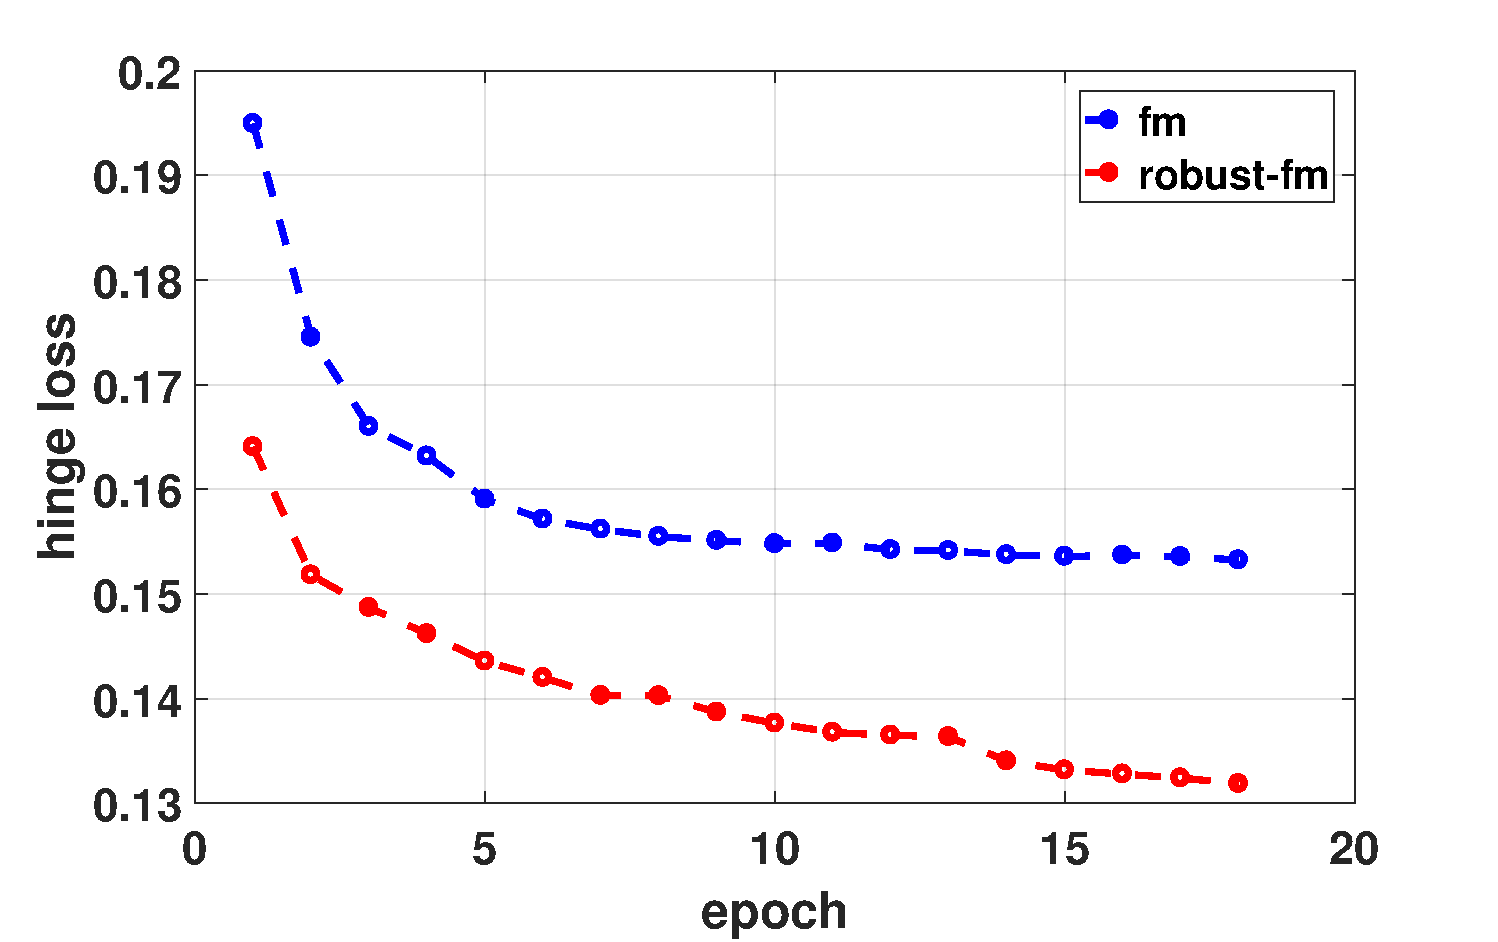
\includegraphics[width=0.48\textwidth]{figs/phishing.pdf}
	}
	\subfigure[w8a]{
		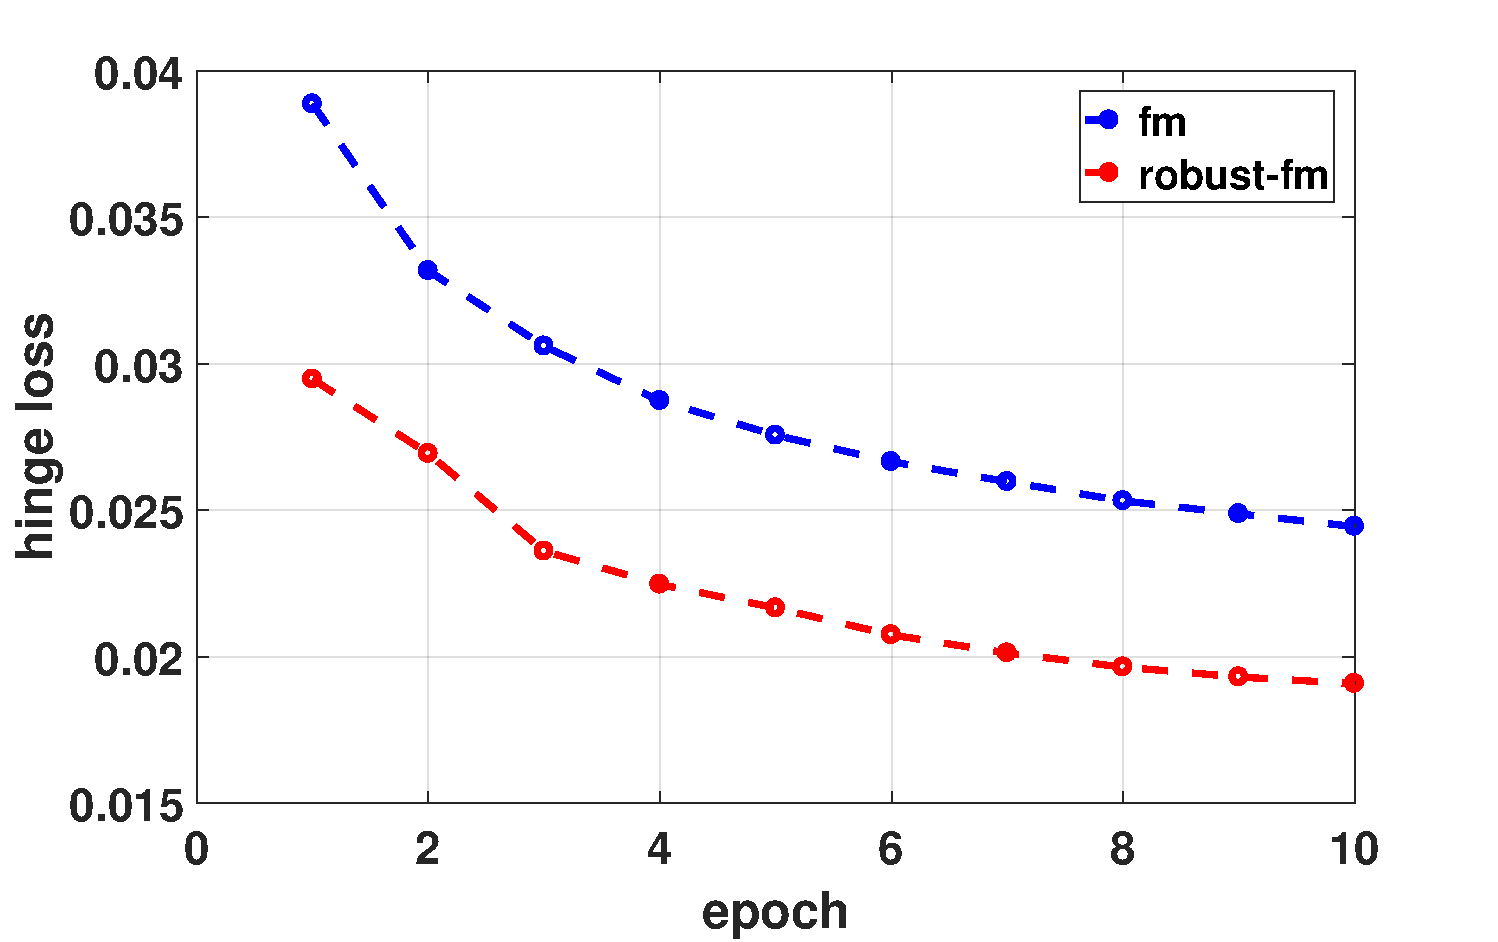
\includegraphics[width=0.48\textwidth]{figs/w8a.pdf}
	}
	\subfigure[IJCNN]{
		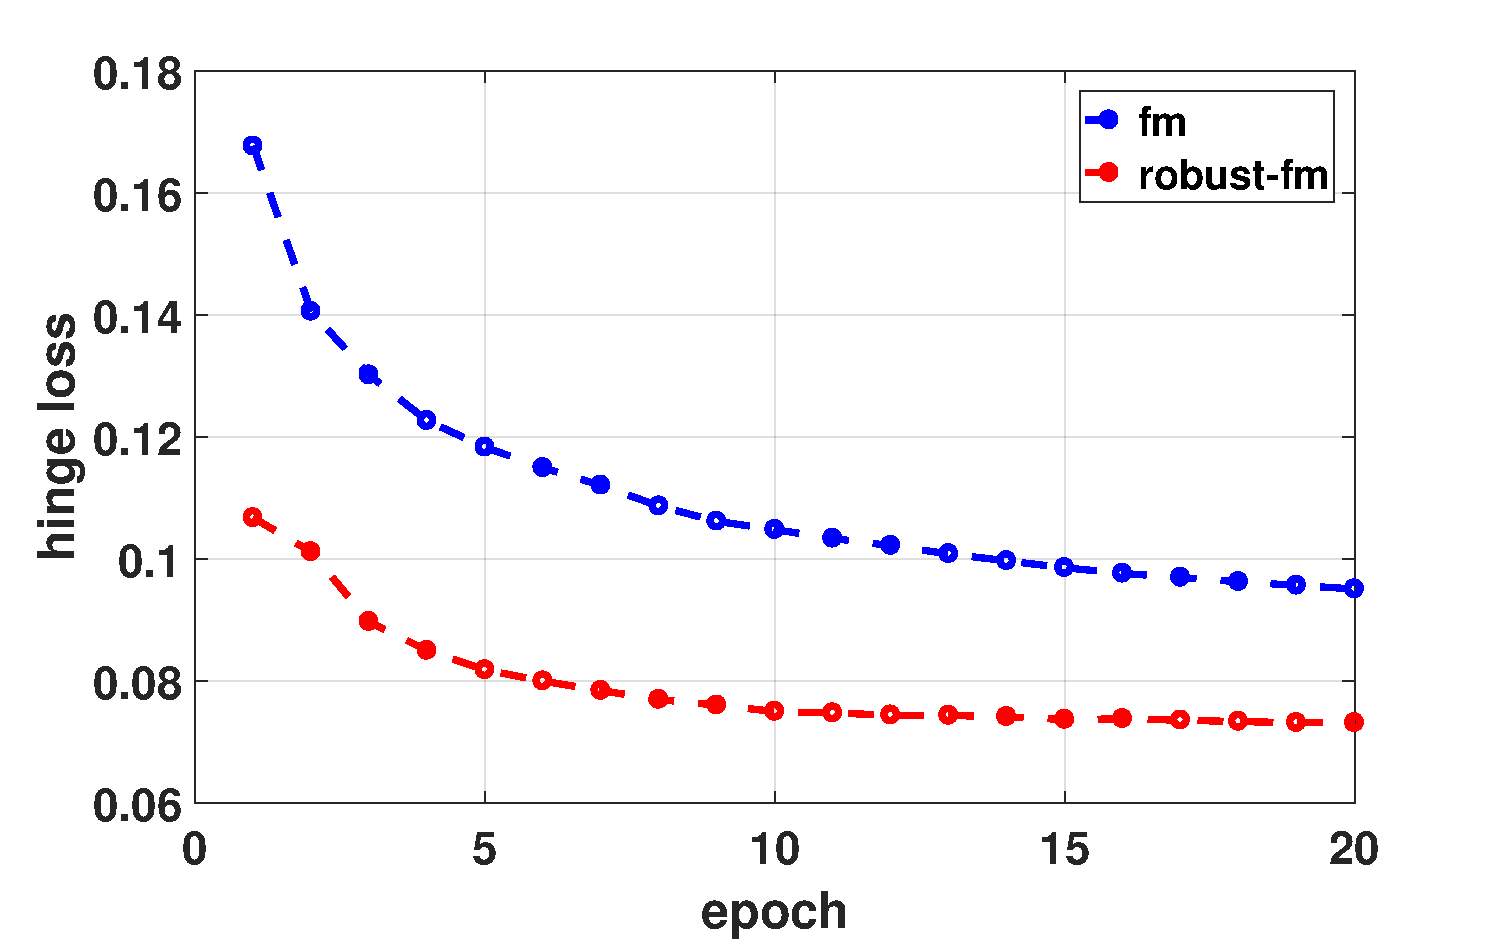
\includegraphics[width=0.48\textwidth]{figs/ijcnn.pdf}
	}
	\subfigure[Covtype]{
		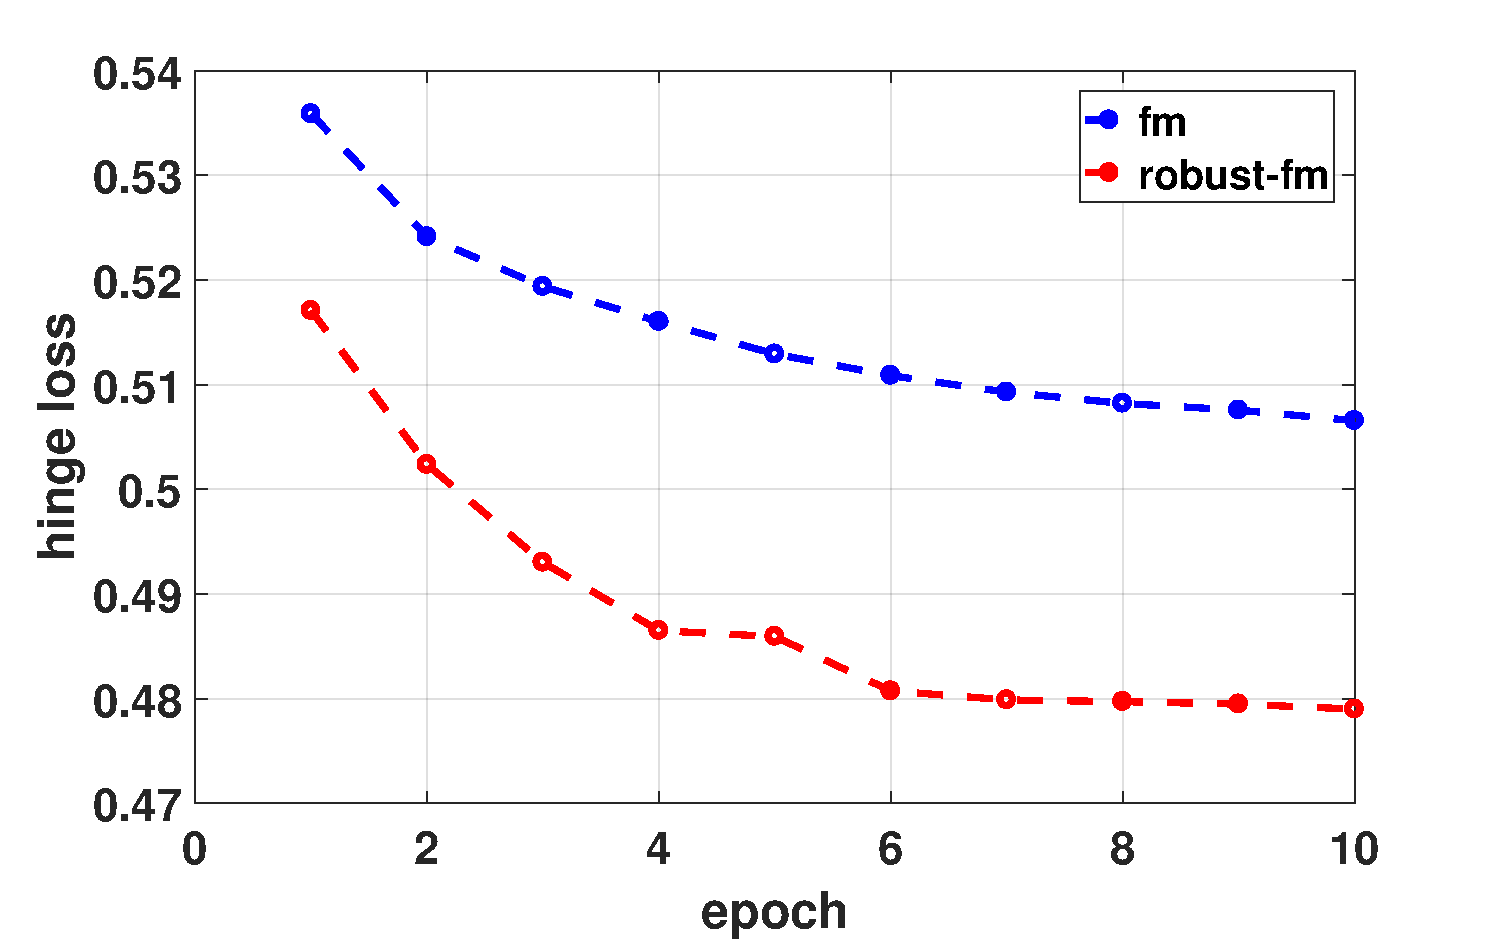
\includegraphics[width=0.48\textwidth]{figs/covtype.pdf}
	}
	\caption{Epoch-wise demonstration of different algorithms with hinge loss on test data}
	\label{allfig}
\end{figure*}

\end{document}
